\section*{Sequence Learning}

\textbf{Sequential data} is data that has a temporal or sequential structure, such as time series, text, or audio. Sequence learning involves modeling this data to capture dependencies and patterns over time.

\subsection*{Recurrent Neural Networks}

RNNs are a family of neural networks designed to handle sequential data. 
\begin{itemize}
  
  \item Recurrent networks take advantage of one of the early ideas found in machine learning: \textbf{parameter sharing}.
  \item If we had separate parameters for each time step, it would be improssible to: (i) generalize to sequence lengths not seen during training (ii) share statistical strength across different sequence lengths/positions in time.
  \item Consider two sentences \enquote{The world faced a pandemic in 2020} and \enquote{In 2020, the world faced a pandemic}.
    \begin{itemize}
      \item \enquote{2020} is a relevant piece of information regardless of its position in the sentence.
      \item A traditional feedforward network would have separate parameters for each position in the sentence, making it difficult to generalize across different positions.
      \item An RNN shares the same weights across several time steps, making it possible to learn patterns that are relevant regardless of their position.
    \end{itemize}
\end{itemize}

\subsection*{Types of RNNs}

\begin{itemize}
  \item \textbf{One-to-one RNNs:} Simplest form, no recurrence. Each input is processed independently, similar to a feedforward neural network.
  \item \textbf{One-to-many RNNs:} Takes a single input and generates a sequence of outputs. Useful for tasks like image captioning.
  \item \textbf{Many-to-one RNNs:} Processes a sequence of inputs and produces a single output. Common in tasks like sentiment analysis.
  \item \textbf{Many-to-many RNNs:} Takes a sequence of inputs and produces a sequence of outputs, where the input and output sequences have the same length. Often used in tasks like speech recognition or named entity recognition.
  \item \textbf{Many-to-many RNNs (encoder-decoder):} A different type of many-to-many RNN where the input and output sequences can have different lengths. Often used in machine translation and other seq-to-seq tasks.
\end{itemize}

\begin{figure}[H]
  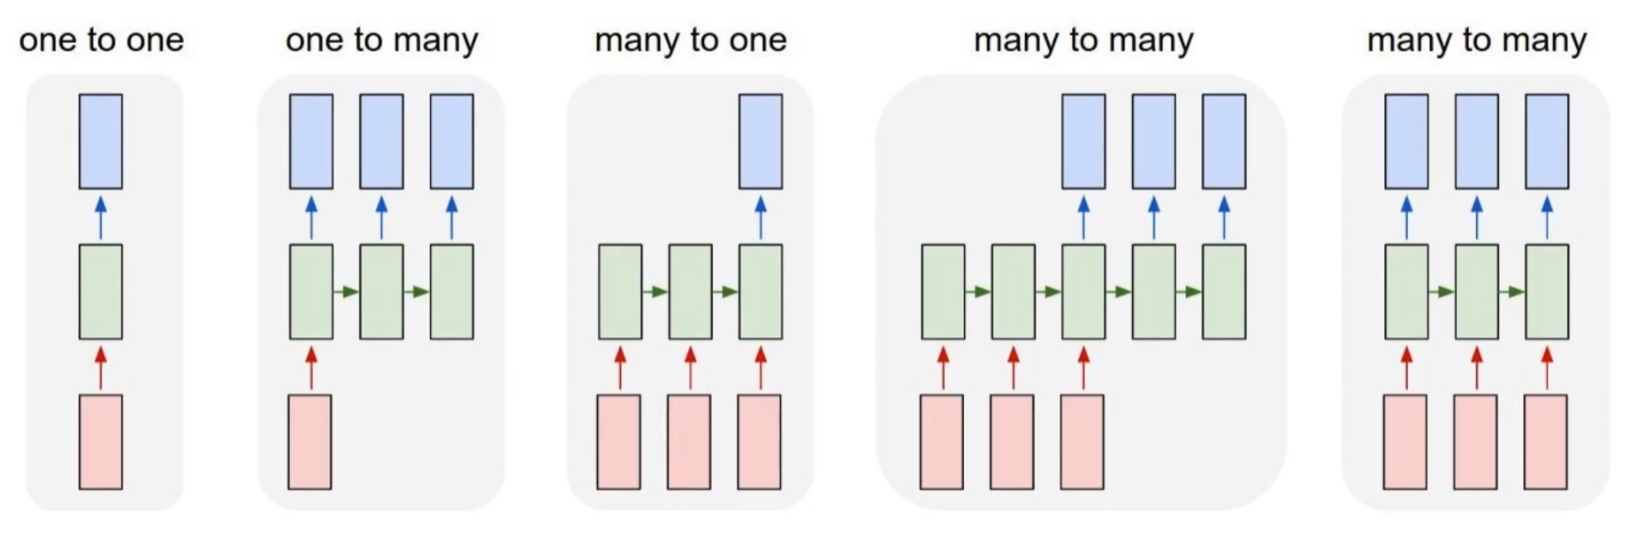
\includegraphics[width=\linewidth]{images/types_of_rnns.png}
\end{figure}

\subsection*{Forward Propagation in RNNs}

\begin{itemize}
  \item At time step $t$, let $\mathbf{x}_t$ be the input, $\mathbf{h}_t$ be the hidden state, and $\mathbf{o}_t$ be the output.
  \item The output $\mathbf{o}_t$ is regarded as giving the unnormalized log probabilities of each possible value of the discrete variable. We can use the softmax function to convert these logits into a vector $\hat{\mathbf{y}}_t$ of probabilities.
  \item For $t = 1, 2, \ldots, \tau$, the forward pass is given by:
    \begin{align*}
      \mathbf{h}^{(t)} &= \text{tanh}(\mathbf{W} \mathbf{h}^{(t-1)} + \mathbf{U} \mathbf{x}^{(t)} + \mathbf{b}) \\
      \mathbf{o}^{(t)} &= \mathbf{V} \mathbf{h}^{(t)} + \mathbf{c} \\
      \mathbf{y}^{(t)} &= \text{softmax}(\mathbf{o}^{(t)})
    \end{align*}
    where $\mathbf{W}$, $\mathbf{U}$, and $\mathbf{V}$ are weight matrices, $\mathbf{b}$ and $\mathbf{c}$ are bias vectors
\end{itemize}

\begin{figure}[H]
  \centering
  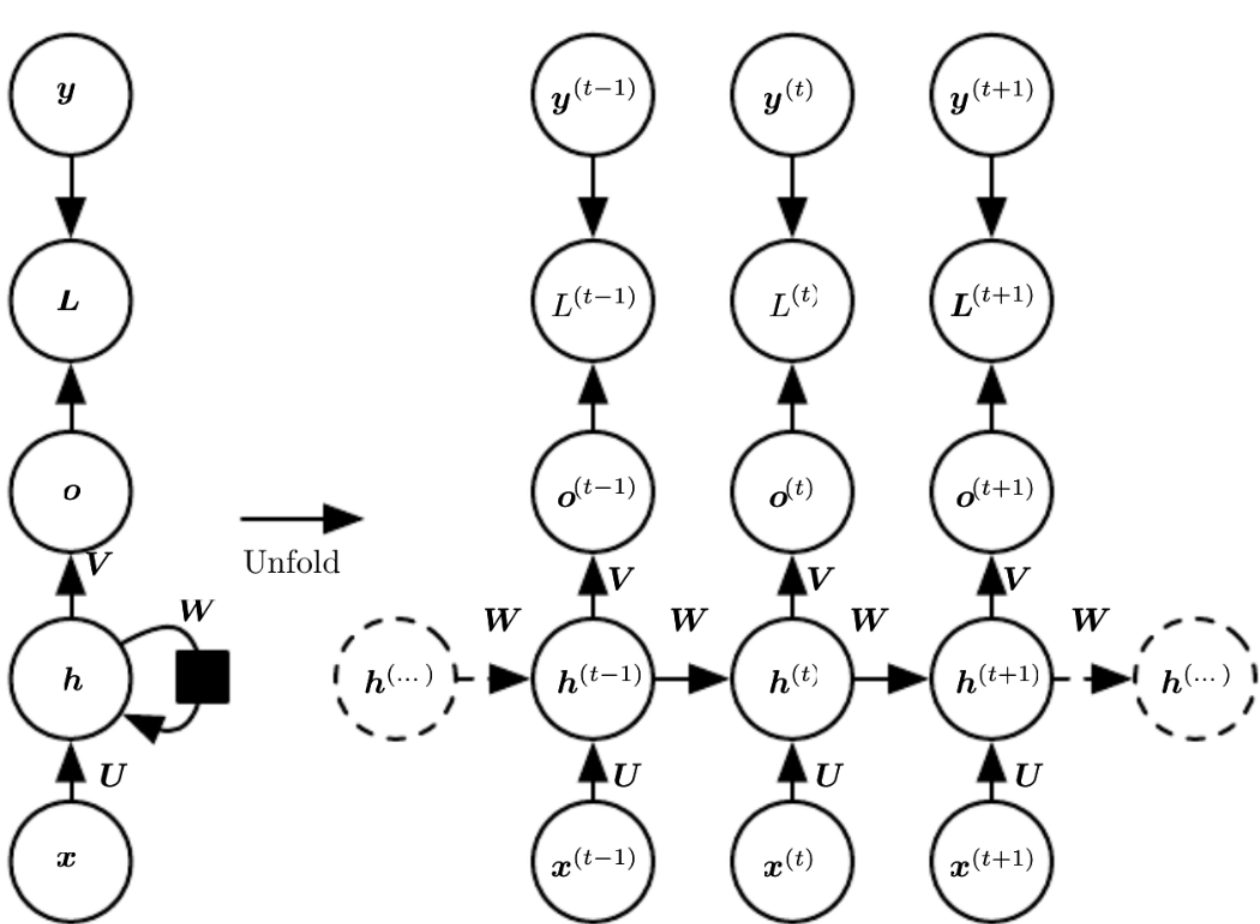
\includegraphics[width=0.8\linewidth]{images/rnn.png}
\end{figure}

\subsection*{Teacher Forcing}

Models that have recurrent connections from the true outputs leading back into the model may be trained using a technique called \textbf{teacher forcing}.

\begin{figure}[H]
  \centering
  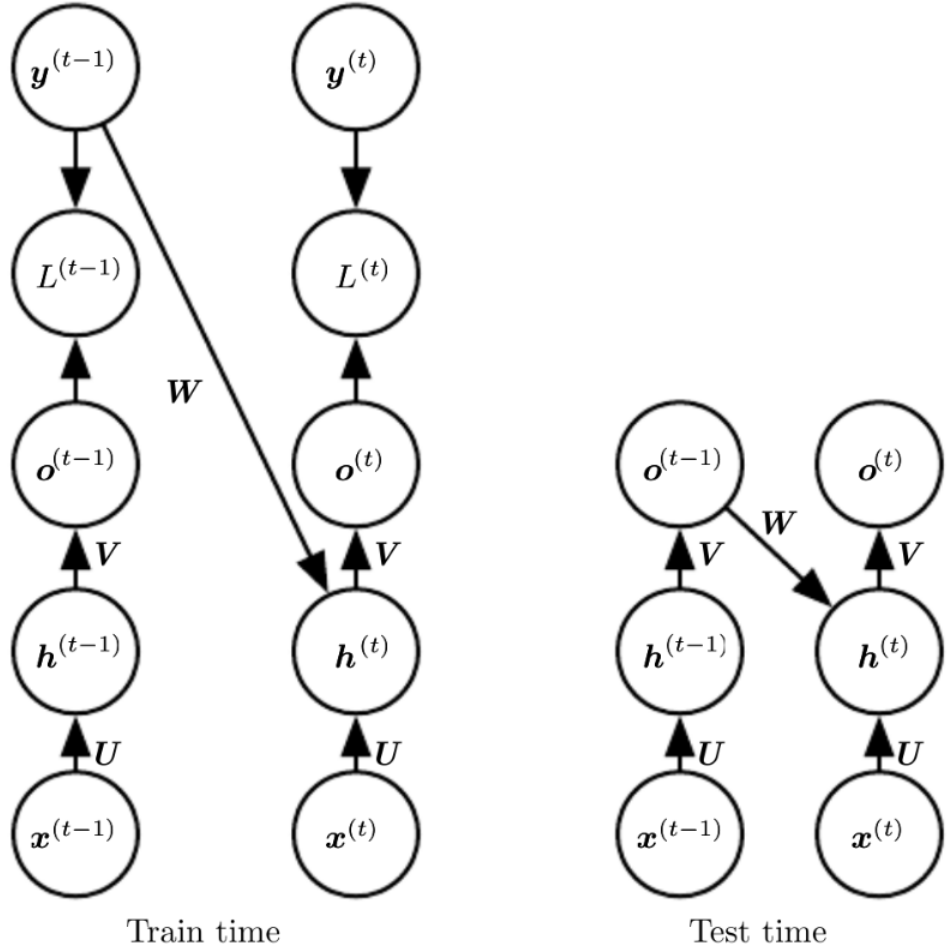
\includegraphics[width=0.7\linewidth]{images/teacher_forcing.png}
  \caption{Teacher forcing. (i) At train time, the \textit{correct output} $\mathbf{y}^{(t)}$ is fed back into the model at the next time step. (ii) At test time, the model's own output ${\mathbf{o}}^{(t)}$ is fed back in as an approximation of the correct output.}
\end{figure}

\subsection*{Challenges in RNNs}

\begin{itemize}
  \item \textbf{Vanishing and Exploding Gradients:} When training RNNs, gradients can either vanish (become too small) or explode (become too large), making it difficult to learn long-term dependencies.
  \item \textbf{Training Time:} RNNs are trained using backpropagation through time (BPTT), which can be computationally expensive and slow, especially for long sequences.
  \item \textbf{Inability to Consider Future Context:} Standard RNNs can only process information in one direction (from past to future). This can be limiting for tasks that require understanding context from both past and future.
\end{itemize}

\subsection*{Long Short-Term Memory}

\textbf{LSTMs} were introduces to address the vanishing gradient problem in RNNs. They use a more complex architecture that includes memory cells and gates to control the flow of information.

\subsubsection*{Differences from RNNs}
\begin{itemize}
  \item Two types of activation functions
  \item A cell state that can carry information across many time steps (\enquote{long-term memory}).
  \item A more complex architecture with three neural networks or \enquote{gates}: (i) forget gate, (ii) input gate, (iii) output gate
  \item An additional network for computing the cell state candidate, which is used to update the cell state.
\end{itemize}

\subsubsection*{Architecture}

\begin{figure}[H]
  \centering
  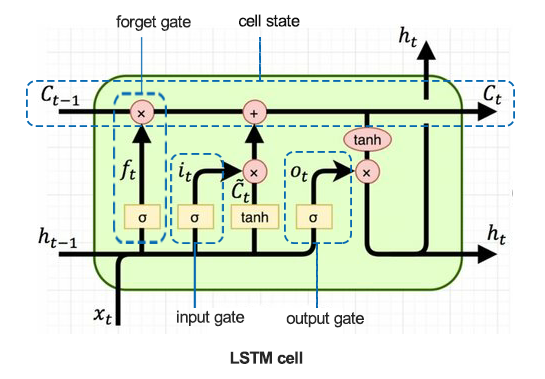
\includegraphics[width=\linewidth]{images/lstm.png}
\end{figure}

\subsection*{Forward Propagation in LSTMs}
In RNNs, the hidden state $\mathbf{h}^{(t)}$ is directly computed from the previous hidden state $\mathbf{h}^{(t-1)}$ and the input $\mathbf{x}^{(t)}$. LSTMs introduce a cell state $\mathbf{c}^{(t)}$ that carries information across many time steps.

At a time step $t$, the forward pass in an LSTM is given by:

\begin{align*}
  \mathbf{i}^{(t)} &= \sigma(\mathbf{W}_i \mathbf{x}^{(t)} + \mathbf{U}_i \mathbf{h}^{(t-1)} + \mathbf{b}_i) & \text{(input gate)} \\
  \mathbf{f}^{(t)} &= \sigma(\mathbf{W}_f \mathbf{x}^{(t)} + \mathbf{U}_f \mathbf{h}^{(t-1)} + \mathbf{b}_f) & \text{(forget gate)} \\
  \tilde{\mathbf{c}}^{(t)} &= \text{tanh}(\mathbf{W}_c \mathbf{x}^{(t)} + \mathbf{U}_c \mathbf{h}^{(t-1)} + \mathbf{b}_c) & \text{(cell state candidate)} \\
  \mathbf{c}^{(t)} &= \mathbf{f}^{(t)} \odot \mathbf{c}^{(t-1)} + \mathbf{i}^{(t)} \odot \tilde{\mathbf{c}}^{(t)} & \text{(cell state update)} \\
  \mathbf{o}^{(t)} &= \sigma(\mathbf{W}_o \mathbf{x}^{(t)} + \mathbf{U}_o \mathbf{h}^{(t-1)} + \mathbf{b}_o) & \text{(output gate)}\\
  \mathbf{h}^{(t)} &= \text{tanh}(\mathbf{c}^{(t)}) \odot \mathbf{o}^{(t)} &\text{ (hidden state)}
\end{align*}


\subsection*{Gated Recurrent Unit}

A \textbf{GRU} uses gates to control the flow of information, similar to LSTMs, but with a simpler architecture.

\subsubsection*{Differences from LSTMs}
\begin{itemize}
  \item Two gates: (i) update gate, (ii) reset gate.
  \item No separate cell state; the hidden state $\mathbf{h}^{(t)}$ carries both short-term and long-term information.
  \item More computationally efficient due to their simpler architecture.
\end{itemize}

\subsubsection*{Architecture}
\begin{figure}[H]
  \centering
  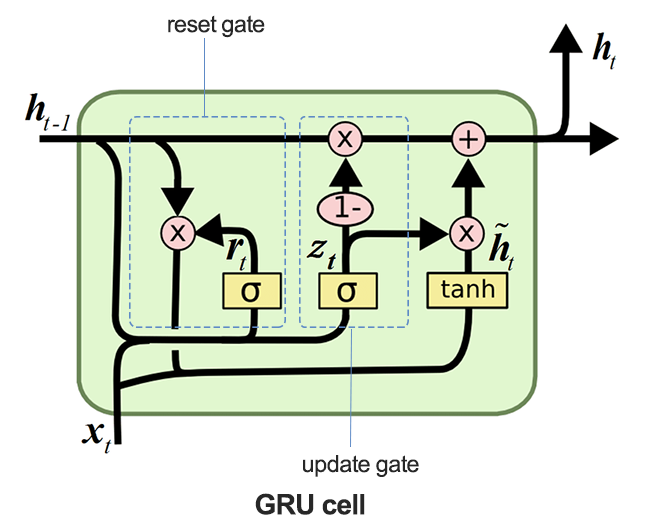
\includegraphics[width=0.7\linewidth]{images/gru.png}
\end{figure}

\subsection*{Forward Propagation in GRUs}
\begin{align*}
  \mathbf{z}^{(t)} &= \sigma(\mathbf{W}_z \mathbf{x}^{(t)} + \mathbf{U}_z \mathbf{h}^{(t-1)} + \mathbf{b}_z) & \text{(update gate)} \\
  \mathbf{r}^{(t)} &= \sigma(\mathbf{W}_r \mathbf{x}^{(t)} + \mathbf{U}_r \mathbf{h}^{(t-1)} + \mathbf{b}_r) & \text{(reset gate)} \\
  \tilde{\mathbf{h}}^{(t)} &= \text{tanh}(\mathbf{W}_h \mathbf{x}^{(t)} + \mathbf{U}_h (\mathbf{r}^{(t)} \odot \mathbf{h}^{(t-1)}) + \mathbf{b}_h) &\text{ (candidate $\mathbf{h}$)} \\
  \mathbf{h}^{(t)} &= (1 - \mathbf{z}^{(t)}) \odot \mathbf{h}^{(t-1)} + \mathbf{z}^{(t)} \odot \tilde{\mathbf{h}}^{(t)} &\text{ (hidden state)}
\end{align*}
